\documentclass[11pt,a4paper]{article}

\usepackage[utf8]{inputenc} % para que nos acepte la codificación UTF-8
\usepackage[spanish]{babel} % establecemos el idioma del documento al español
\usepackage[colorlinks=true,linkcolor=magenta]{hyperref} % para poder poner "enlaces" en nuestro codigo
\usepackage{color} % para darle color a nuestros documentos
\usepackage{enumerate} % para poder añadirle a enumerate un argumento con el tipo de "contador" que queremos
\usepackage{multirow} % para hacer tablas con mas de una columna
\usepackage{amsmath} % paquete basico de matematicas
\usepackage{minted} % para resaltar código fuente
\usepackage{graphicx} % para incluir imágenes en nuestro código
\usepackage{fancyhdr} % para personalizar la cabecera y el pie de pagina
\usepackage{lastpage} % para saber el numero de pagina del documento

\pagestyle{fancy}

% CABECERA
\fancyhead[LE,RO]{\textcolor[rgb]{0.5,0.2,0.6}{Marta Gómez}} % el nombre del autor en la izquierda de las paginas pares y a la derecha de las paginas impares
\fancyhead[RE,LO]{\textcolor[rgb]{0.2,0.2,0.9}{\date{\today}}} % en el lado contrario, la fecha

% PIE DE PAGINA
\fancyfoot[C]{\textcolor[rgb]{0.2,0.4,0.5}{\thepage{} de} \pageref{LastPage}} % en la parte central del pie de pagina el numero de pagina actual y un enlace a la ultima pagina

% para importar código fuente desde ficheros externos en c++
\newmintedfile[mycplusplus]{c++}{
    linenos, % muestra el número de línea
    numbersep=5pt, % separación entre el código y el número de línea
    gobble=0, % columna desde la que empieza a mostrar código
    frame=lines, % dibuja las líneas enmarcando el código
    framesep=2mm, % separación entre la línea y el código
    tabsize=3, % tamaño de la tabulación
}

\begin{document}
% especificamos el titulo del documento y le ponemos un tamaño de letra grande
\title{\huge Portafolios de prácticas}
% Y ahora, el autor
\author{Marta Gómez}
% le añadimos la fecha actual
\date{\today}

\maketitle % nos crea el titulo, el autor y la fecha en el inicio del documento
\tableofcontents % nos crea un indice con enlaces a las diferentes secciones y subsecciones

\setcounter{section}{-1} % el contador de secciones empieza en 0
\section{Descripción del programa}
\subsection{Funcionamiento del programa}
\noindent
El programa da al usuario a elegir entre escribir en la \textit{entrada estándar} una operación aritmética en \textbf{notación postfija} o \textbf{notación infija} y después, devuelve el resultado de dicha operación por la \textit{salida estándar}.

\noindent
La siguiente tabla refleja la diferencia entre notación postfija y notación infija:

\begin{tabular}{|p{4cm} | p{4cm} |}
\hline % para poner una linea horizontal
Notación infija & Notación postfija \\ % el & se usa para separar columnas y el \\ para saltos de linea
\hline
$1 + 2$ & $1$ $2 +$ \\
$5 + ((1 + 2) * 4) - 3$ &  $5$ $1$ $2 + 4 * + 3 -$ \\
\hline
\end{tabular}

\noindent
Las distintas estructuras que hay en el fichero son:

\begin{enumerate}[1.]
	\item \textbf{clase Postfija}: que contiene los siguientes métodos:
	\begin{itemize}
		\item Constructor
		\item Método que calcula el resultado de la operación.
	\end{itemize}
	\item \textbf{función infija2postfija}: función que pasa de infija a postfija.
\end{enumerate}

\newpage % para empezar una nueva página
\section{Código del programa}
\noindent
El código en C++ de la clase Postfija y la función infija2postfija es el siguiente: \label{codigo_programa}
\mycplusplus[label="postfija.h"]{postfija.h}

\newpage
\section{Análisis de la eficiencia del programa}
\noindent
En primer lugar, nos encontramos un for que va desde $i=0$ hasta $s.size()$, donde $s.size()$ es el tamaño de string que contiene la operación aritmética en notación infija. Este for equivaldría a la siguiente sumatoria, si todas las operaciones dentro de dicho for fueran de eficiencia $O(1)$:

\begin{displaymath}
\sum_{i=0}^{s.size()} = 1 = s.size(), \qquad\ \textrm{siendo $s.size()$ el tamaño del string que contiene la operación aritmética}
\end{displaymath}

\noindent
Ahora, vamos a proceder a analizar las operaciones dentro de dicho for:
\begin{enumerate}[$\heartsuit$]
	\item Tenemos en primer lugar una asignación, cuya eficiencia es $O(1)$
	\item Y después un if, como sabemos las comparaciones también tienen $O(1)$, y dentro de dicho if una llamada a una función que lo único que hace es añadir un elemento a la cola, por lo que también es $O(1)$.
	\item Luego tenemos un else, cuyas operaciones también tienen un coste de $O(1)$ puesto que tanto Pila como Cola están implementadas con celdas enlazadas.
\end{enumerate}

\noindent
Por tanto, tal y como dijimos antes, la eficiencia del bucle es de $O(s.size())$.

\noindent
Después, tenemos un pequeño bucle, en el que insertamos en la cola de la operación postfija, los operadores con menos prioridad que han quedado en la pila. Este bucle iría desde $0$ hasta $t$, siendo $t$ el tamaño de la pila. Y se traduciría en la siguiente sumatoria:

\begin{displaymath}
\sum_0^t 1 = t
\end{displaymath}

\noindent
Por último,  tenemos otro bucle más en el que metemos en un string la operación en notación postfija que hemos calculado y lo devolvemos. La devolución tiene eficiencia $O(1)$, y las operaciones que hacemos dentro del bucle también, por tanto, el bucle se traduciría en la siguiente sumatoria:

\begin{displaymath}
\sum_{i=0}^{c.size()} 1 = c.size();
\end{displaymath}

\subsection{Conclusión}
Tenemos tres bucles, al ser independientes, la eficiencia de todo el código es la suma de la eficiencia de cada bucle por separado, es decir:

\begin{displaymath}
eficiencia = \underbrace{s.size() + t + c.size()}_{O(n)} = O(n)
\end{displaymath}

\noindent
Podemos concluir diciendo que la eficiencia de nuestra función es $O(n)$.

\newpage
\section{Salida del programa}
\noindent
La salida por terminal que obtener al ejecutar el \hyperref[codigo_programa]{programa} es la siguiente:

\begin{figure}[!h]
\centering
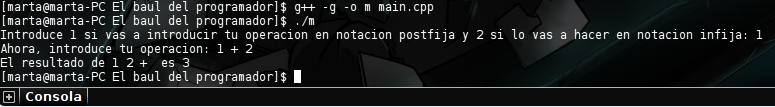
\includegraphics[width=1\textwidth]{1}
\caption{Salida por terminal del programa}
\end{figure}

\end{document}
